%!TEX root = main.tex

\section{Simulation}

\label{sec:simulation}

\subsection{Simulation setup}
In this section, we study the performance of the smart explicitness congestion notification mechanism we proposed using ndnSim\cite{ndnsimnet, ndnsim}.

Fig.~\ref{fig-topology} shows the network topology we use in the simulation. There are two topologies we use. One is bottleneck topology and the other one is mesh topology. In both network topologies, there are many consumers who send Interest into network and retrieve the corresponding Data from the producer. The number of consumers varies from 1 to 100, and each consumer requests Data with a same prefix (means they are a same flow). In the mesh network, consumers can get Data from three paths and each path's bottleneck bandwidth is different. Each link's capacity varies from 30~Mbps to 200~Mbps and the propagation delay of each hop is 10~ms. The buffer in each node is equal to the production of bandwidth and delay. In the following figures, the bandwidth means the bottleneck's bandwidth.

We set the value of $\alpha$ and $\beta$ as 0.2 and 1.5 respectively. We compare our smart-ECN with ICP and ICP-shape. ICP is a TCP-style Interest control protocol in NDN. The Interest sending window is passively changed according the RTT and loss of Data, following the AIMD principle\cite{ICP}. ICP-shape also follows the AIMD principle but it discards the Interest instead Data when the routers sense congestion\cite{improveshape}. ICP-shape also sends NACK back to receiver if an Interest is shaped. NACK is a feedback information used to inform that the Interest has been discarded or there's no Data corresponding to the Interest. The consumer should retransmit the same Interest when it receives a NACK.

Our simulation includes three parts. In the first part we evaluate the flow number estimating process, which we propose in Eq.~\ref{eq:flownum}. In the second part, we will evaluate the ECN Interest sending rate mechanism using the bottleneck network topology. At last we will estimate the smart forwarding mechanism using the mesh network topology. The simulation result shows the number flows can be estimated accurately. Compared with ICP and ICP-shape, ECN Interest sending rate mechanism performance better in link utilization, packets dropping and flow complete time. Our smart forwarding mechanism has better TFCT compared with adaptive forwarding mechanism.

\begin{figure}[t]
\centering
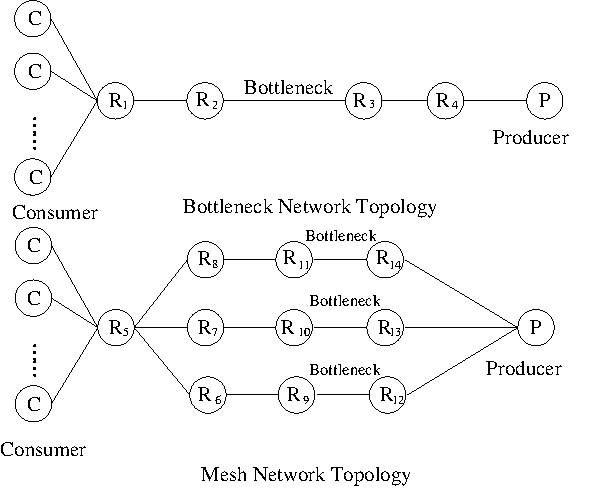
\includegraphics[width=3in]{topology.pdf}
\caption{The two network topologies using in simulation.}
\label{fig-topology}
\end{figure}

\subsection{The estimated flow number}

By Eq.~\ref{eq:flownum}, the flow number of the link can be estimated by the rate of this link. The size of Data can be estimated as the average size of the Data that goes through. Under the bottleneck network topology, at t=0, 10 flows start. At t=10 another 10 flows start. And at t=20, 10 flows finish, there are only 10 flows left. From Fig.~\ref{fig-flownum} we can see that the flow number can be accurately estimated. Even when the flow number changes, the estimation can also converge.

\begin{figure}[t]
\centering
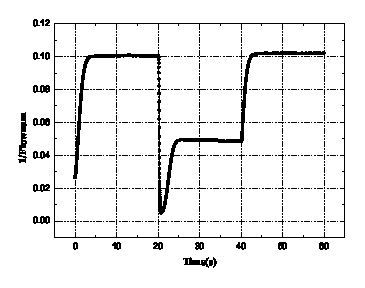
\includegraphics[width=2.5in]{flownum-pic-cut.eps}
\caption{The accuracy of estimation of flow number.}
\label{fig-flownum}
\end{figure}

\subsection{The performance of ECN Interest sending rate mechanism}

We use bottleneck topology to estimate the ECN Interest sending rate mechanism. The ECN Interest sending rate is calculated based on the principle that the bandwidth should be fully used. The ICP and ICP-shape use the TCP-style window control way. TCP-style window control way uses the timeout-principle to sense the congestion, and once timeout, it cut the interest window to half. TCP-style window control also use the slow-start to send the Interest. These will waste a lot of bandwidth. As Fig.~\ref{fig-linkuti} shows, ICP and ICP-shape waste bandwidth because of the slow start. The link utilization of ICP and ICP-shape is between 80\%-90\%. In contrast, even when the bottleneck link's bandwidth changes, the bandwidth utilization by smart-ECN always closes to 100\%.

\begin{figure}[t]
	\centering
	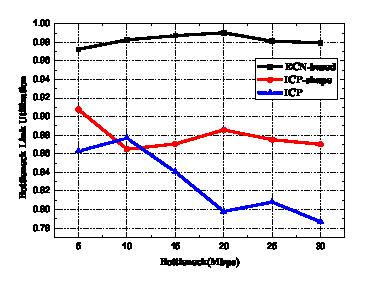
\includegraphics[width=2.5in]{utilization-pic-cut.eps}
	\caption{The bottleneck's link utilization compared with ICP and ICP-shape when change the bottleneck bandwidth.}
	\label{fig-linkuti}
\end{figure}

Because the ECN Interest sending rate makes sure that the rate can not exceed the bandwidth, almost no packets (no matter Interest or Data) drop in ECN interest sending rate mechanism, as the Fig.~\ref{fig-drop} shows. ICP uses timeout as the signal to inform congestion, and timeout is caused by dropping Data. In ICP, once the link become congested, the only solution is to drop Data, so the number of dropped Data is very large, as Fig.~\ref{fig-drop} shows. The ICP-shape shapes Interest before congestion happens, so it can reduce the number of Data needed to be dropped because of congestion. But as the delay of sending back and the difficulty of estimating the congestion, there are still some dropped Data.

\begin{figure}[t]
	\centering
	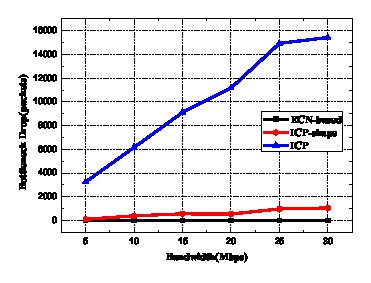
\includegraphics[width=2.5in]{drop-pic-cut.eps}
	\caption{The number of dropping packets in bottleneck compared with ICP and ICP-shape when change the bottleneck bandwidth.}
	\label{fig-drop}
\end{figure}

As Eq.~\ref{eq:updated_rt5} shows, the packets in the queue should do the utmost to be drained. This principle makes sure that in smart-ECN, the packets in the queue are always close to 0, as shown in Fig.~\ref{fig-queue}. In ICP, to use the bandwidth effectively, the receivers always try to enlarge the Interest window until the Data fills up the queue and the Data is dropped, so the packets in the queue is large. In ICP-shape, the router can shape Interest when it sense that congestion will happen. So in ICP-shape, the queue size is smaller than ICP, as shown in Fig.~\ref{fig-queue}.

\begin{figure}[t]
	\centering
	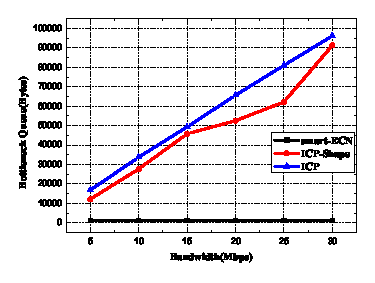
\includegraphics[width=2.5in]{queu-pic-cut.eps}
	\caption{The volume of queuing packets in bottleneck compared with ICP and ICP-shape when change the bottleneck bandwidth.}
	\label{fig-queue}
\end{figure}

Fig.~\ref{fig-fct} shows the FCT of different flows. Flow complete time in NDN is defined as the time from when receiver sends the first Interest until the receiver receives the last Data of the flow. The ECN Interest sending rate mechanism's link utilization is much higher than ICP. ECN Interest sending rate mechanism fairly applies bandwidth resource to all the flows, so even if the short flow can get fair bandwidth resource. No matter flows are short or long, their FCT are much better than ICP, as Fig.~\ref{fig-fct} shows.

\begin{figure}[t]
	\centering
	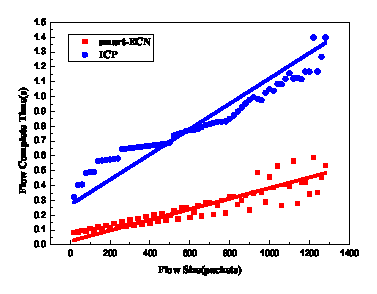
\includegraphics[width=2.5in]{fct-cut.eps}
	\caption{Smart-ECN's flow complete time compared with ICP.}
	\label{fig-fct}
\end{figure}

\subsection{Flow complete time compared with ICP}

We demonstrate the effectiveness of smart adaptive forwarding mechanism using mesh network topology. The total bottleneck bandwidth means the sum of bottleneck bandwidth on all the available paths. Using the forwarding-assistance and route information, the smart adaptive forwarding mechanism can choose a network-wide best path. The adaptive mechanism chooses the best forwarding interface just by the next hop's link information. As the next hop link information can not reflect the whole path's information, the adaptive mechanism will sometimes choose a wrong path whose later link is shared by far more flows. The non-adaptive \red{(change without to non in Fig.~\ref{fig-tfct})} mechanism chooses the path just by the route information, similar with TCP/IP. The non-adaptive mechanism can not change the forwarding interface according the network condition. As Fig.~\ref{fig-tfct} shows, under different total bandwidth, the smart adaptive forwarding's TFCT is much better than non-adaptive mechanism. As smart adaptive forwarding mechanism can choose a best path on the network-wide view, it's total flow complete time is even better than adaptive mechanism.

\begin{figure}[t]
	\centering
	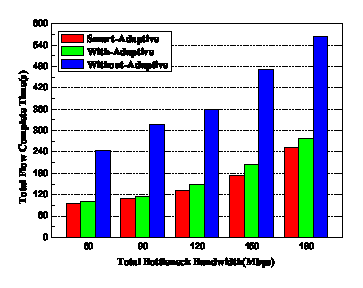
\includegraphics[width=2.5in]{adaptive-pic-cut.eps}
	\caption{Total flow complete time compared with other two forwarding mechanisms.}
	\label{fig-tfct}
\end{figure}
